\documentclass{article}
\usepackage{graphicx}
\usepackage[utf8]{inputenc}
\usepackage[english]{babel}
 
\usepackage{color}
 
\newcommand{\ale}{\color{red}}

\begin{document}

\title{ \textbf{ Search for WIMP inelastic scattering off xenon nuclei with XENON100} \\  Response on Referee report -- DE12171/Aprile  }
%\author{}

\maketitle


%\section{Introduction}
%Here is the text of your introduction.

We thank the referee for the valuable comments, we sincerely think these added value to the paper.  We addressed all the comments and implemented most of the suggestions in the new version of the manuscript. Below we list each comment/question in blue and its related answer in black, and we specifically state which modifications
were implemented in the new version of the paper.

\begin{itemize}
	\item {\color{blue} General: are these new SD limits isospin independent, applying to both protons and neutrons, unlike the traditional elastic SD for dark matter? If so, should be indicated right off the bat in the abstract.}
\end{itemize}

The new SD limits are indeed isospin dependent, we followed the literature and Ref. [6] and set limits on spin-dependent, WIMP-neutron interactions. Isospin independent constraints could be the subject of a different publication.

\begin{itemize}
	\item {\color{blue} Introduction, third paragraph: Can you add a sentence further
elucidating how it is possible for dark matter, of the masses and
cross-sections you probe in this paper, to fail to be detected through
elastic scattering, given current existing world-best limits from
XENON1T and LUX and PandaX, yet still be possible through inelastic?
It was still unclear to me. Basically, I want to understand if there
was any reasonable scenario under which you could have seen a signal, or
whether that was already impossible and you were doomed to only set
a limit. This changes the theme of the paper significantly in my mind
from discovery potential to a confirmation/cross-check of an existing
limit in a new channel. - “10 keV of deposited energy: Does this
refer to nuclear or electron recoil or both? Unclear since we are now
dealing with inelastic scattering that produces a gamma too here.}
\end{itemize}

Classical searches for spin-dependent elastic scattering have higher sensitivity compared to this search for 
spin-dependent inelastic scattering. However, in case dark matter would be found, a positive signal in the inelastic channel would deliver a clear evidence for  
the spin-dependent nature of the interaction. 
In the text we mention that this search is complementary to the standard SD search.  We modified the text to "It was found that this channel,  
although not competitive in terms of sensitivity,  
is complementary to the spin-dependent, elastic scattering one".
The "10\,keV" of deposited energy refers to both; if one looks at integrated rated above 10\,keV NR for elastic scattering, one  
finds that is below the integrated rate of  NR+ER for inelastic scattering, see Fig. 6 in (https://arxiv.org/abs/1309.0825).
We think that deposited energy is the correct wording here, since indeed it differs for the two cases.

\begin{itemize}
	\item {\color{blue} 
Section III: Is there a reason the complete 477 live-days cannot be
used for this paper? Wouldn’t this make your constraints even
stronger? Please explain reason}
\end{itemize}

Yes, the limit would have been stronger, a naive expectation for the sensitivity improvement with respect to the current one is $\sim$30\%.
However the main scope of this paper is to explore a different analysis channel, and not to improve the sensitivity for SD searches, as mentioned above.
Combining three different science runs (each acquired under different background conditions and with different acceptances) is very demanding,
and would have extended significantly the time scale for this analysis. Such an extension  was not well-motivated at the time given the fact that XENON1T was to start data taking soon.


\begin{itemize}
	\item {\color{blue} 
III.B: How were the ROI limits chosen? Text doesn’t say: should
explain, are these +/- some number of sigma relative to the expected
means of the NR and ER in cS1 and cS2 space?}
\end{itemize}

The signal distribution changes with the WIMP mass due to the NR component.
We selected the ROI such that it will contain the WIMP hypothesis at least at two 
sigma. This statement is now added to the text.


\begin{itemize}
	\item {\color{blue} 
While I understand the sub-regions were chosen to have roughly equal
number of events, it is not very clear to me at all why there are so
many different ones, and why there seems to be no rhyme or reason to
their sizes/shapes. It is also unclear, especially since Figure 1a is
an example of only one mass (100 GeV WIMP) how these regions were
picked to be optimal for any WIMP mass studied, doesn’t seem to be
possible to me. (Lastly, why didn’t you just take equal slices in S1
and S2 and make squares for example?)}
\end{itemize}

\begin{figure}[t!]
  \centerline{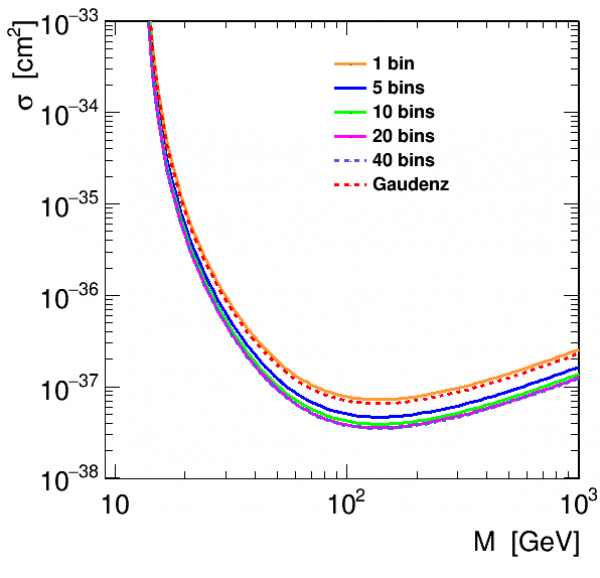
\includegraphics[width=0.7\linewidth]{inelastic_binning_check.png}}
  \caption{ Sensitivity computed dividing the ROI in different numbers of equally sized bins. Please note: these sensitivity curves where obtained in a test long before the final version, most of nuisance parameter have  a different implementation or are missing, hence they are not directly comparable with the final one, although similar.}
  \label{fig:binning}
\end{figure}

If one follows an appropriate binning procedure, then the choice of bins is irrelevant, meaning that 
the final result should not depend on the binning. Furthermore, we did not specify that this particular 
choice is optimal for all WIMP masses.

We have shown, please see Figure~\ref{fig:binning}, that once we divide the region in more than 10 equally sized bins,
the difference in sensitivity is small. Hence, as soon as we divide the ROI in any number $>$10 of equally sized bins, we practically obtain the same result. 
%So why not divide in 40 equally sized bins at this point?  
%There is a limiting factor: we are using asymptotic formulae for distribution of the
%test statistic, these formulae are valid in the assumption of Wilks theorem, so that the number
%of events in each bin should be "large". In order to not have bins with dramatically low background, which
%happens in case of equally sized bins, we needed to merge bins and we need to do it in a way to not disrupt sensitivity.
We selected a rebinning strategy that depends on the background shape and is the same for all masses. The bin shapes are designed to have
equal background density: this ensures high discrimination power while keeping a low number of bins and ensures that all bins are 
well populated (this assumption is necessary for the used test statistic asymptotic formulae). 
%So we started with a number of equally sized bins (roughly 20 if I remember correctly) and we grouped them achieving similar 
%background density,  in this way the discrimination power is conserved, meaning that the discrimination power will be equal or better than 
%the one using the same number of final bins (in this case 9) but produced in equal sizes.
%Within this prescription, which is very general, the chosen arrangement of bins and shapes is almost arbitrary and
%could have been done in many different ways, however it doesn't matter because following 
%this procedure whatever peculiar binning choice will not  impact  our 
%sensitivity, so we choose the solution that was technically easier.
We added to the text that "it has been cross-checked that changing the bin choice does not impact the sensitivity".


\begin{itemize}
	\item {\color{blue} 
Multiple-scatter cut: While I understand the cut on a second largest
peak, what happens when the peaks from multiple scatters are merged
because they are too close together? Also, the language is slightly
unclear: does “regardless of S2 signal size” mean the primary S2 peak,
or all peaks added together in a given event, counting them all as
“the signal”?}
\end{itemize}

Our detector position resolution is of the order of a few mm, multiple-scatter S2s that are 
closer than the resolution will be merged. These present however not a problem for our analysis, since this cut is designed 
to reduce the neutron background. In the standard elastic analysis this turns into a small
uncertainty in neutron background model, but for the energy deposits of this analysis the neutron background 
is irrelevant (hence we could have even dropped this selection criterium). When we say S2 we mean the primary peak. 

\begin{itemize}
	\item {\color{blue} 
Figure 2 caption slightly unclear: I assume the figures include both
the ER and the NR associated with the inelastic scatter, and not just
the former as the text implies. Please correct, to better match up
with explanation below in Section C.}
\end{itemize}

Indeed, and we changed to "a full simulation (NR and ER response) of the 39,6\,keV xenon line..." 

\begin{itemize}
	\item {\color{blue} 
Equation 2: It is not clear where S1 photon detection efficiency gets
folded in here: currently this equation appears to yield photons not
PE (Ly?) Am I reading it incorrectly?}
\end{itemize}

Ly is the measured light yield in PE/keV$_{ee}$, hence it contains the position dependence
and the collection efficiencies of the signal, as described in more detail in 
(https://arxiv.org/abs/1207.3458). This notation is common to XENON papers, but it might not be 
general.


\begin{itemize}
	\item {\color{blue} 
~0.80 +/- 0.05: Given the importance of knowing the final signal
acceptance fraction I don’t understand why this has a “$\simeq$,” especially
since error bars are provided. Why is this still approximate? It
should not be, unless you meant it changes with WIMP mass, and in that
case a range should be provided, from the min to max masses you
considered.}
\end{itemize}

This is correct, and we changed to: "The combined acceptance  of all selection criteria in the region 
of interest is roughly constant for all masses and averages to $(0.80\pm0.05)$."



\begin{itemize}
	\item {\color{blue} 
Section D: seems odd, doesn’t seem to add much beyond C and Figure 2.
If there is no new information here, please remove it, or at reduce
the length of the paragraph to include only those, and merge with C.
Weird to have a section be one short paragraph by itself.}
\end{itemize}


We agree, and section D has now been merged to section C.



\begin{itemize}
	\item {\color{blue} 
E: It is not clear to me how 60Co and 232Th calibrations can tell you
the BG in the signal region, given they have different energy
spectra/distributions than BG? Isn’t it better to validate the
simulation for 60Co and 232Th then simulate using NEST for example
events of the same energy distribution as your actual ER BG? In fact,
the BG simulation here seems to contradict the signal simulation in
the earlier section. Why the dichotomy in methods, especially since
the 39.6 keV line was actually present in calibration data, and so
this all seems backwards to me. This could explain your unresolved
systematic in F. you write is outside statistical fluctuation
expectation. (You should have a BG prior from counting the parts of
XENON100 and simulating in Geant4, yes?)}
\end{itemize}


It has been shown in several XENON analyses that indeed $^{60}$Co and $^{232}$Th are good
representations of the ER background at low energies, since they reproduce well the Compton-scatter band. They have been used several  times, 
see for example (https://arxiv.org/abs/1207.3458, and https://arxiv.org/abs/1609.06154).
A full simulation with NEST will not give smaller uncertainties due to intrinsic
NEST uncertainties and due to the  uncertainty in the MC prediction of the radiogenic neutron background from materials.
Furthermore, we do not have a full MC-data matching for XENON100 at these energies, 
meaning we don't have a Geant4-based model of all the material 
backgrounds that produces spectra that we can fully trust. Hence we opted for a simple 
but effective approach. 
Regarding the "dichotomy of treatment": we could not use AmBe data as a signal model due to 
the non-negligible difference between WIMP and AmBe introduced by the mass-dependent NR.


\begin{itemize}
	\item {\color{blue} 
Figure 3: statistical and systematic uncertainties should be denoted
separately as is more standard practice, either splitting them off or
using color coded error bars, as you do later}
\end{itemize}

Since we use a large MC sample the statistical uncertainties are negligible, the bin with the largest uncertainty 
has  a relative error of $<$1\%. This makes the statistical uncertainty smaller than the thickness of the line.
We thus removed the "statistical" uncertainty label, as here we aim to underline the systematic uncertainties.


\begin{itemize}
	\item {\color{blue} Pseudo-samples: I am confused as to why these are necessary, doesn’t
the ROOT PLR function allow profiling out over multiple such
systematic uncertainties simultaneously and continuously, and not just
in discrete +/-1-sigma steps? You also should explain whether
parameters are all railed to their plus/minus 1-sigma’s all together
or separately? This could be over-conservative, or swing the other
way, depending on the correlations on these parameters, which I know
for a fact myself can be very tricky: for example, raising a light
yield can be canceled out by lowering light collection efficiency,
each within its respective uncertainties, and not necessarily in
integer multiples of their standard deviations of course. This sounds
to me like what would be done in an “enhanced” cut-and-count-style
analysis, but not in a PLR. Perhaps it is because you did binned and I
am used to using PLR continuous (unbinned)? Can you please clarify,
and justify your choice of binned versus unbinned? This goes back to
my original question about the 9 strange sub-regions: How, a priori,
were they selected, optimized, and validated? How does one choose
one’s bins? Was it blind? Speaking of which, it should be made clear
what was blind or not in the text. I imagine not much since you are
primarily an NR-search experiment and this has ER Bottom of p. 6: How
can all parameters related to systematics be justified as normal, as
opposed to Poisson or skewed-normal in at least some cases? What I
mean is, for example a low-energy NR with a very low expected number
of photons detected is not going to have a symmetric distribution,
since there is no such thing as a negative number of photons. Does not
apply to higher energies, but I thought you have low O(10 keV) from
the NR here too Figure 4: minor comment, but sentences just a bit out
of order. Last sentence should move earlier because it refers to
discussion about the top half of the figure.}
\end{itemize}

This comment touches many topics and we try to reply to each in the following:
\begin{enumerate}
	\item Regarding the pseudo-samples, these are used to produce the shape uncertainty, hence histogram variation, in $\pm$1-sigma steps. One typically uses these "pseudo-samples" histograms  as seeds for interpolation techniques controlled by a nuisance parameter, as the referee suggest. We have several such shape uncertainties and we felt that this approach was over complicated. We opted for a conservative but simple approximation: we sum up in quadrature all the "positive" and "negative" variations for each bin separately, we then assign the maximal of the two as a symmetric Gaussian distributed uncertainty on the single bin.  In this way we avoid the complication of histogram shape interpolation of several nuisance parameter. As the uncertainty in each bin is independent from one another, this allows for more freedom and has over coverage of the shape variations.
	
	\item The question on the regions is already answered above. 
	
	\item Since this parameter space in the data was explored in several other studies, our analysis was not blind.
		Nonetheless, the employed analysis procedure was as if the signal region were blind, since we didn't tune our event selection criteria on the data in the ROI.

	\item All the systematic uncertainties come from auxiliary measurements, either from our experiment or from the literature, so 
		to the best of our knowledge their prior is indeed a Gaussian. 
		However, some of these may not be expected to feature a Gaussian distribution, for example L$_{\rm{eff}}$, but in these cases the chosen parameterisation
		is the one commonly accepted in the field.

	\item We agree, and the sentences in the caption of Figure 4 have been swapped.
\end{enumerate}





\begin{itemize}
	\item {\color{blue} Section IV: Please briefly define in text the difference between CL(s)
and the more common CL, and add a sentence explaining the benefit of
CL(s), or at least a brief reason why it was used instead of CL. Not
all readers may be familiar with Read’s work.}
\end{itemize}

We agree, and the sentence   "The CL$_s$ technique helps to protect against excluding  a cross section which is smaller than the experimental sensitivity."  has been added.



\begin{itemize}
	\item {\color{blue} 
Figure 5: Was the result constrained, due to large BG
under-fluctuation, to be at -1-sigma-level, as it appears to be in
this figure? If so, this should be stated in the figure caption and/or
text and explained. Also, based on flat regions I see in the 1- and
2-sigma bands in the plot it appears as though the limit was smoothed,
but the bands were not. Both should be left as raw data points, or
both smoothed, please choose, but be consistent (personally I prefer
smooth, but a definite case can be made for discrete connected by
straight lines in log-log in between the individual mass points you
actually run in your PLR; past XENON and LUX and other results vary in
choice of what to do in a case like this). This discrepancy is most
noticeable between 100 and 200 GeV, where the blue bands are extremely
straight, while the limit is curved. Lastly, are there really no other
results to put on this plot? Not even an earlier XENON one? This is
very surprising, but it does underscore the significance of your work
here, as being in nearly virgin territory, and you can say that.}
\end{itemize}

No the limit is not constrained, CLs is used instead of a power constrained limit.
It is simply a coincidence that it stops at -1 sigma.
The referee is correct, the bands are not smoothened while the curve is -  this is due to a ROOT 
problem (smoothening of a filled area does not work well in ROOT) which we  
fixed now. 
There is no other result that we know of which explores 
exactly this inelastic scattering process. In particular, this is the first time we analysed the XENON data for 
such a signature (we note that new structure function calculations were only available in 2013).




\end{document}

